\documentclass[a4paper,pdftex]{article}

\usepackage{array}
%\usepackage{mathtools}
\usepackage{hopsantut}
\usepackage{listings}
\usepackage{todonotes}
\usepackage[fleqn]{amsmath}
\usepackage{tikz}

\hypersetup{pdfauthor={Robert Braun and Peter Nordin}, pdftitle={Hopsan Tutorial - Writing Advanced Components}, pdfsubject={Hopsan Tutorial}}

\lstset{ %
  numbers			=	left,
  numberstyle		=	\scriptsize, % the style that is used for the line-numbers
  backgroundcolor	=\color{yellow!10}
}

\begin{document}
\maketitle{Writing Advanced Components}

\section*{Introduction}
This tutorial is a continuation of the \textit{Writing Component Libraries} tutorial. It explains how to write more advanced components based on acausal equations and physical connections. It also covers how to re-write the equations for the impedance variables, which are a consequence of the transmission line element method.

Two components are explained; a variable pump component with linear equations, and a translational mass component with second order dynamics.

\section*{Requirements}
It is necessary to know how to write and compile components for Hopsan, either using HoLC or a third-party tool. This is covered by the \textit{Writing Component Libraries} tutorial.

\section*{Hydraulic Pump}
A hydraulic pump is a component that transforms an angular velocity on a shaft into hydraulic flow. In this case we will use a simple model with no dynamics, where the angular velocity is assumed to be constant at all time. This is similar to the Q-Type Variable Displacement Pump component in the Hopsan default library.

The component is shown in the figure below. It consists of two hydraulic ports for inlet and outlet, respectively. It also has four input variables; displacement ($D$), displacement setting ($\varepsilon$), angular velocity ($\omega$) and leakage coefficient ($c_{leak}$). All of these 

\begin{tikzpicture}
\node[] () {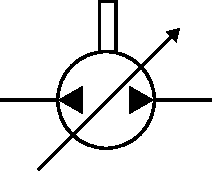
\includegraphics{gfx/writingadvancedcomponents/variablepump.pdf}};
\node[yshift=5pt] () {$D$};
\node[yshift=-20pt, xshift=3pt] () {$C_{leak}$};
\node[yshift=33pt, xshift=40pt] () {$\varepsilon$};
\node[yshift=50pt, xshift=1pt] () {$n$};
\node[yshift=-7pt, xshift=-60pt] () {$p_{1}$};
\node[yshift=-7pt, xshift=60pt] () {$p_{2}$};
\node[xshift=36pt] () {$q$};
\draw[very thick, ->] (25pt,-7pt) -> (44pt,-7pt);
\end{tikzpicture}

\subsection*{Equations}
The flow from a hydraulic pump can be modelled with the following equations:

\begin{equation*}
\begin{cases}
q - q_{leak} = \varepsilon D \omega/2\pi \\
q_{leak} = C_{leak}\Delta p
\end{cases}
\end{equation*}

Here $q$ is the generated flow and $q_{leak}$ the leakage flow. $\Delta p$ is the pressure difference over the pump. In Hopsan we will have one flow and pressure at each port. Thus, we need to introduce the variables $p_{1}$ and $q_{1}$ for the inlet port, and $p_{2}$ and $q_{2}$ for the outlet. Flow is always defined as positive outwards from Q-type components. Therefore, the inlet flow will be the same as the outlet flow but negative. The equations now become:

\begin{equation*}
\begin{cases}
q_{2} - C_{leak}(p_{1}-p_{2}) = \varepsilon D \omega/2\pi \\
q_{1} = -q_{2}
\end{cases}
\end{equation*}

However, Hopsan uses the transmission line element method. For this reason we will not get the pressure variables as explicit input variables. Instead, we get a \textit{wave variable} and an \textit{impedance}. The TLM equations are then used to calculate the pressures from the flow variables, according to the two new equations below:

\begin{equation*}
\begin{cases}
q_{2} - C_{leak}(p_{1}-p_{2}) = \varepsilon D \omega/2\pi \\
q_{1} = -q_{2}\\
p_{1} = c_{1} + q_{1}Z_{c,1}\\
p_{2} = c_{2} + q_{2}Z_{c,2}
\end{cases}
\end{equation*}

It is now possible to rearrange the equations so that the can be solved analytically. First we replace the pressure variables in the first equation with the TLM equations:

\begin{equation*}
\begin{cases}
q_{2} - C_{leak}(c_{1} - q_{2}Z_{c,1}-c_{2} - q_{2}Z_{c,2}) = \varepsilon D \omega/2\pi \\
q_{1} = -q_{2}\\
p_{1} = c_{1} + q_{1}Z_{c,1}\\
p_{2} = c_{2} + q_{2}Z_{c,2}
\end{cases}
\end{equation*}

Finally, we rearrange the first equation to break out the flow variable:

\begin{equation*}
\begin{cases}
q_{2} = (\varepsilon D \omega/2\pi - C_{leak}(c_{1} -c_{2})) / (1-C_{leak}(Z_{c,1}-Z_{c,2}))\\
q_{1} = -q_{2}\\
p_{1} = c_{1} + q_{1}Z_{c,1}\\
p_{2} = c_{2} + q_{2}Z_{c,2}
\end{cases}
\end{equation*}

We now have a linear equation system that can be solved step-by-step. 

\subsection*{C++ Code}

\begin{minipage}{\linewidth}
\begin{lstlisting}[basicstyle=\footnotesize\ttfamily]
#include "ComponentEssentials.h"

namespace hopsan {

class HydraulicFixedDisplacementPump : public ComponentQ
{
private:
    double *mpND_p1, *mpND_q1, *mpND_c1, *mpND_Zc1; 
    double *mpND_p2, *mpND_q2, *mpND_c2, *mpND_Zc2;
    double *mpW, *mpDp, *mpClp, *mpEps;
    Port *mpP1, *mpP2;

public:
    static Component *Creator()
    {
        return new HydraulicFixedDisplacementPump();
    }
\end{lstlisting}
\end{minipage}

\begin{minipage}{\linewidth}
\begin{lstlisting}[basicstyle=\footnotesize\ttfamily]
void configure()
{
    mpP1 = addPowerPort("P1", "NodeHydraulic");
    mpP2 = addPowerPort("P2", "NodeHydraulic");

	addInputVariable("eps", "Displacement setting", "", 1.0, &mpEps);
    addInputVariable("w_p", "Angular Velocity", "rad/s", 250.0, &mpW);
    addInputVariable("D_p", "Displacement", "m^3/rev", 0.00005, &mpDp);
    addInputVariable("C_lp", "Leakage Coeff.", "(m^3/s)/Pa", 0.0, &mpClp);
}
\end{lstlisting}
\end{minipage}

\begin{minipage}{\linewidth}
\begin{lstlisting}[basicstyle=\footnotesize\ttfamily]
void initialize()
{
    mpND_p1 = getSafeNodeDataPtr(mpP1, NodeHydraulic::Pressure);
    mpND_q1 = getSafeNodeDataPtr(mpP1, NodeHydraulic::Flow);
    mpND_c1 = getSafeNodeDataPtr(mpP1, NodeHydraulic::WaveVariable);
    mpND_Zc1 = getSafeNodeDataPtr(mpP1, NodeHydraulic::CharImpedance);

    mpND_p2 = getSafeNodeDataPtr(mpP2, NodeHydraulic::Pressure);
    mpND_q2 = getSafeNodeDataPtr(mpP2, NodeHydraulic::Flow);
    mpND_c2 = getSafeNodeDataPtr(mpP2, NodeHydraulic::WaveVariable);
    mpND_Zc2 = getSafeNodeDataPtr(mpP2, NodeHydraulic::CharImpedance);
}
\end{lstlisting}
\end{minipage}

\begin{minipage}{\linewidth}
\begin{lstlisting}[basicstyle=\footnotesize\ttfamily]
void simulateOneTimestep()
{
    //Declare local variables
    double p1, q1, c1, Zc1, p2, q2, c2, Zc2;

    //Read input variables
    double w = (*mpW);
    double dp = (*mpDp);
    double Clp = (*mpClp);
    double eps = (*mpEps);

    //Get variable values from nodes
    c1 = (*mpND_c1);
    Zc1 = (*mpND_Zc1);
    c2 = (*mpND_c2);
    Zc2 = (*mpND_Zc2);

    //Fixed Displacement Pump equations
    q2 = ( dp*eps*w/(2.0*pi) + Clp*(c1-c2) ) / ( (Zc1+Zc2)*Clp+1 );
    q1 = -q2;
    p2 = c2 + Zc2*q2;
    p1 = c1 + Zc1*q1;

    //Check for cavitation
    bool cav = false;
    if (p1 < 0.0)
    {
        c1 = 0.0;
        Zc1 = 0.0;
        cav = true;
    }
    if (p2 < 0.0)
    {
        c2 = 0.0;
        Zc2 = 0.0;
        cav = true;
    }
    if (cav)
    {
        q2 = ( dp*eps*w/(2.0*pi) + Clp*(c1-c2) ) / ( (Zc1+Zc2)*Clp+1 );

        p1 = c1 + Zc1 * q1;
        p2 = c2 + Zc2 * q2;
        if (p1 <= 0.0)
        {
            p1 = 0.0;
            q2 = std::min(q2, 0.0);
        }
        if (p2 <= 0.0)
        {
            p2 = 0.0;
            q2 = std::max(q2, 0.0);
        }
        q1 = -q2;
    }

    //Write new values to nodes
    (*mpND_p1) = p1;
    (*mpND_q1) = q1;
    (*mpND_p2) = p2;
    (*mpND_q2) = q2;
}
\end{lstlisting}
\end{minipage}

\section*{Translational Mass}

\subsection*{Equations}

\subsection*{C++ Code}
 	
\end{document}